% Group 1: figures from figures/lok/
\begin{figure}[htbp]
    \centering
    \includegraphics[width=1.2\textwidth, bb=0 0 800 800, clip]{figures/lok/histogram.jpeg}
    \caption{Histogram illustrating the distribution of effective parties for mountain and plain constituencies}
    \label{img:histogram}
\end{figure}

\begin{figure}[htbp]
    \centering
    \includegraphics[width=1.2\textwidth, bb=0 0 800 800, clip]{figures/lok/mountain_states.jpeg}
    \caption{Mountain states: Effective parties for each state}
    \label{img:mountain_enp}
\end{figure}

\begin{figure}[htbp]
    \centering
    \includegraphics[width=1.2\textwidth, bb=0 0 800 800, clip]{figures/lok/plains_states.jpeg}
    \caption{Plain states: Effective parties for each state}
    \label{img:plain_enp}
\end{figure}

\begin{figure}[htbp]
    \centering
    \includegraphics[width=1.2\textwidth, bb=0 0 800 800, clip]{figures/lok/final.jpeg}
    \caption{Mountain states v/s Plain States: Effective parties for entire regions}
    \label{img:overall_enp}
\end{figure}

% Group 2: figures from figures/assembly/
\begin{figure}[htbp]
    \centering
    \includegraphics[width=0.9\textwidth, bb=0 0 800 800, clip]{figures/assembly/histogram.jpeg}
    \caption{Histogram illustrating the distribution of effective parties for mountain and plain constituencies}
    \label{img:assembly_histogram}
\end{figure}

\begin{figure}[htbp]
    \centering
    \includegraphics[width=0.9\textwidth, bb=0 0 800 800, clip]{figures/assembly/assembly_elections_mountain_states.jpeg}
    \caption{Mountain states: Effective parties for each state}
    \label{img:assembly_mountain_enp}
\end{figure}

\begin{figure}[htbp]
    \centering
    \includegraphics[width=0.9\textwidth, bb=0 0 800 800, clip]{figures/assembly/assembly_elections_plains_states.jpeg}
    \caption{Plain states: Effective parties for each state}
    \label{img:assembly_plain_enp}
\end{figure}

\begin{figure}[htbp]
    \centering
    \includegraphics[width=0.9\textwidth, bb=0 0 800 800, clip]{figures/assembly/assembly_final_adjusted.jpeg}
    \caption{Mountain states v/s Plain States: Effective parties for entire regions}
    \label{img:assembly_overall_enp}
\end{figure}

% Group 3: figures from figures/nfhs/ using forced placement
\begin{figure}[H]
    \centering
    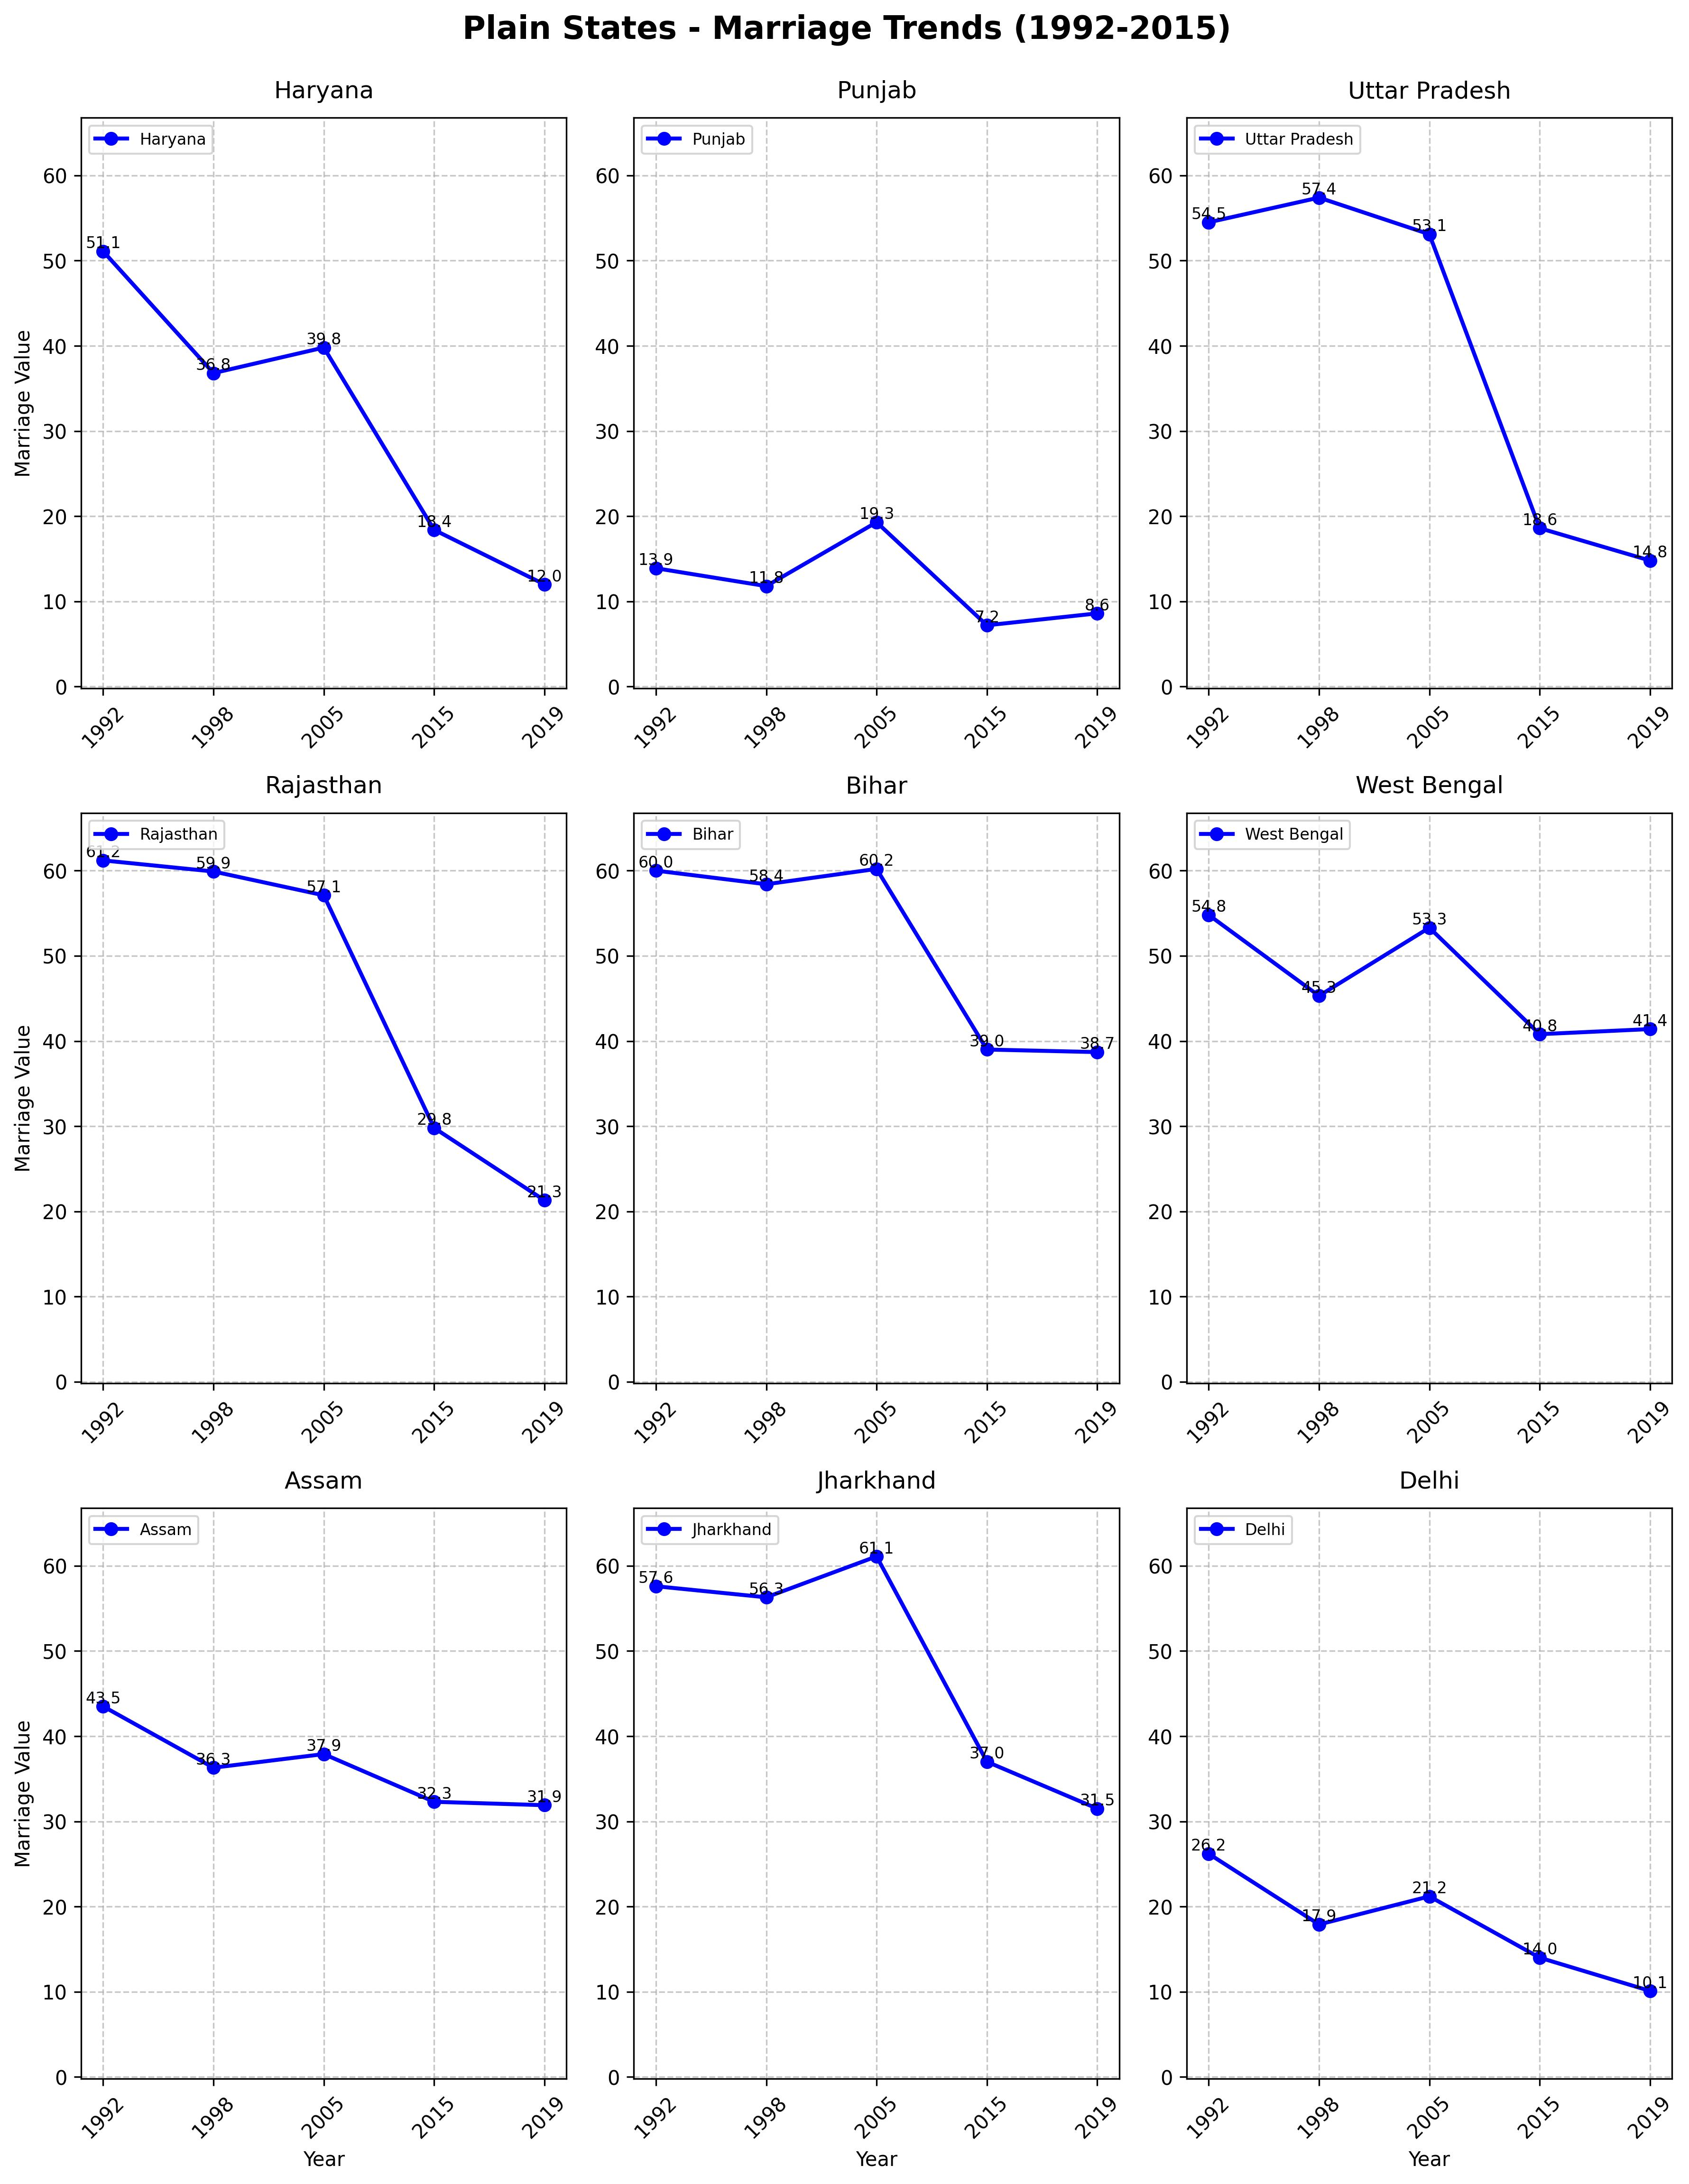
\includegraphics[width=0.9\textwidth, bb=0 0 800 800, clip]{figures/nfhs/plain_states_marriage_subplots.jpeg}
    \caption{Child Marriage age in Plain States}
    \label{fig:nfhs_plain_marriage}
\end{figure}

\begin{figure}[H]
    \centering
    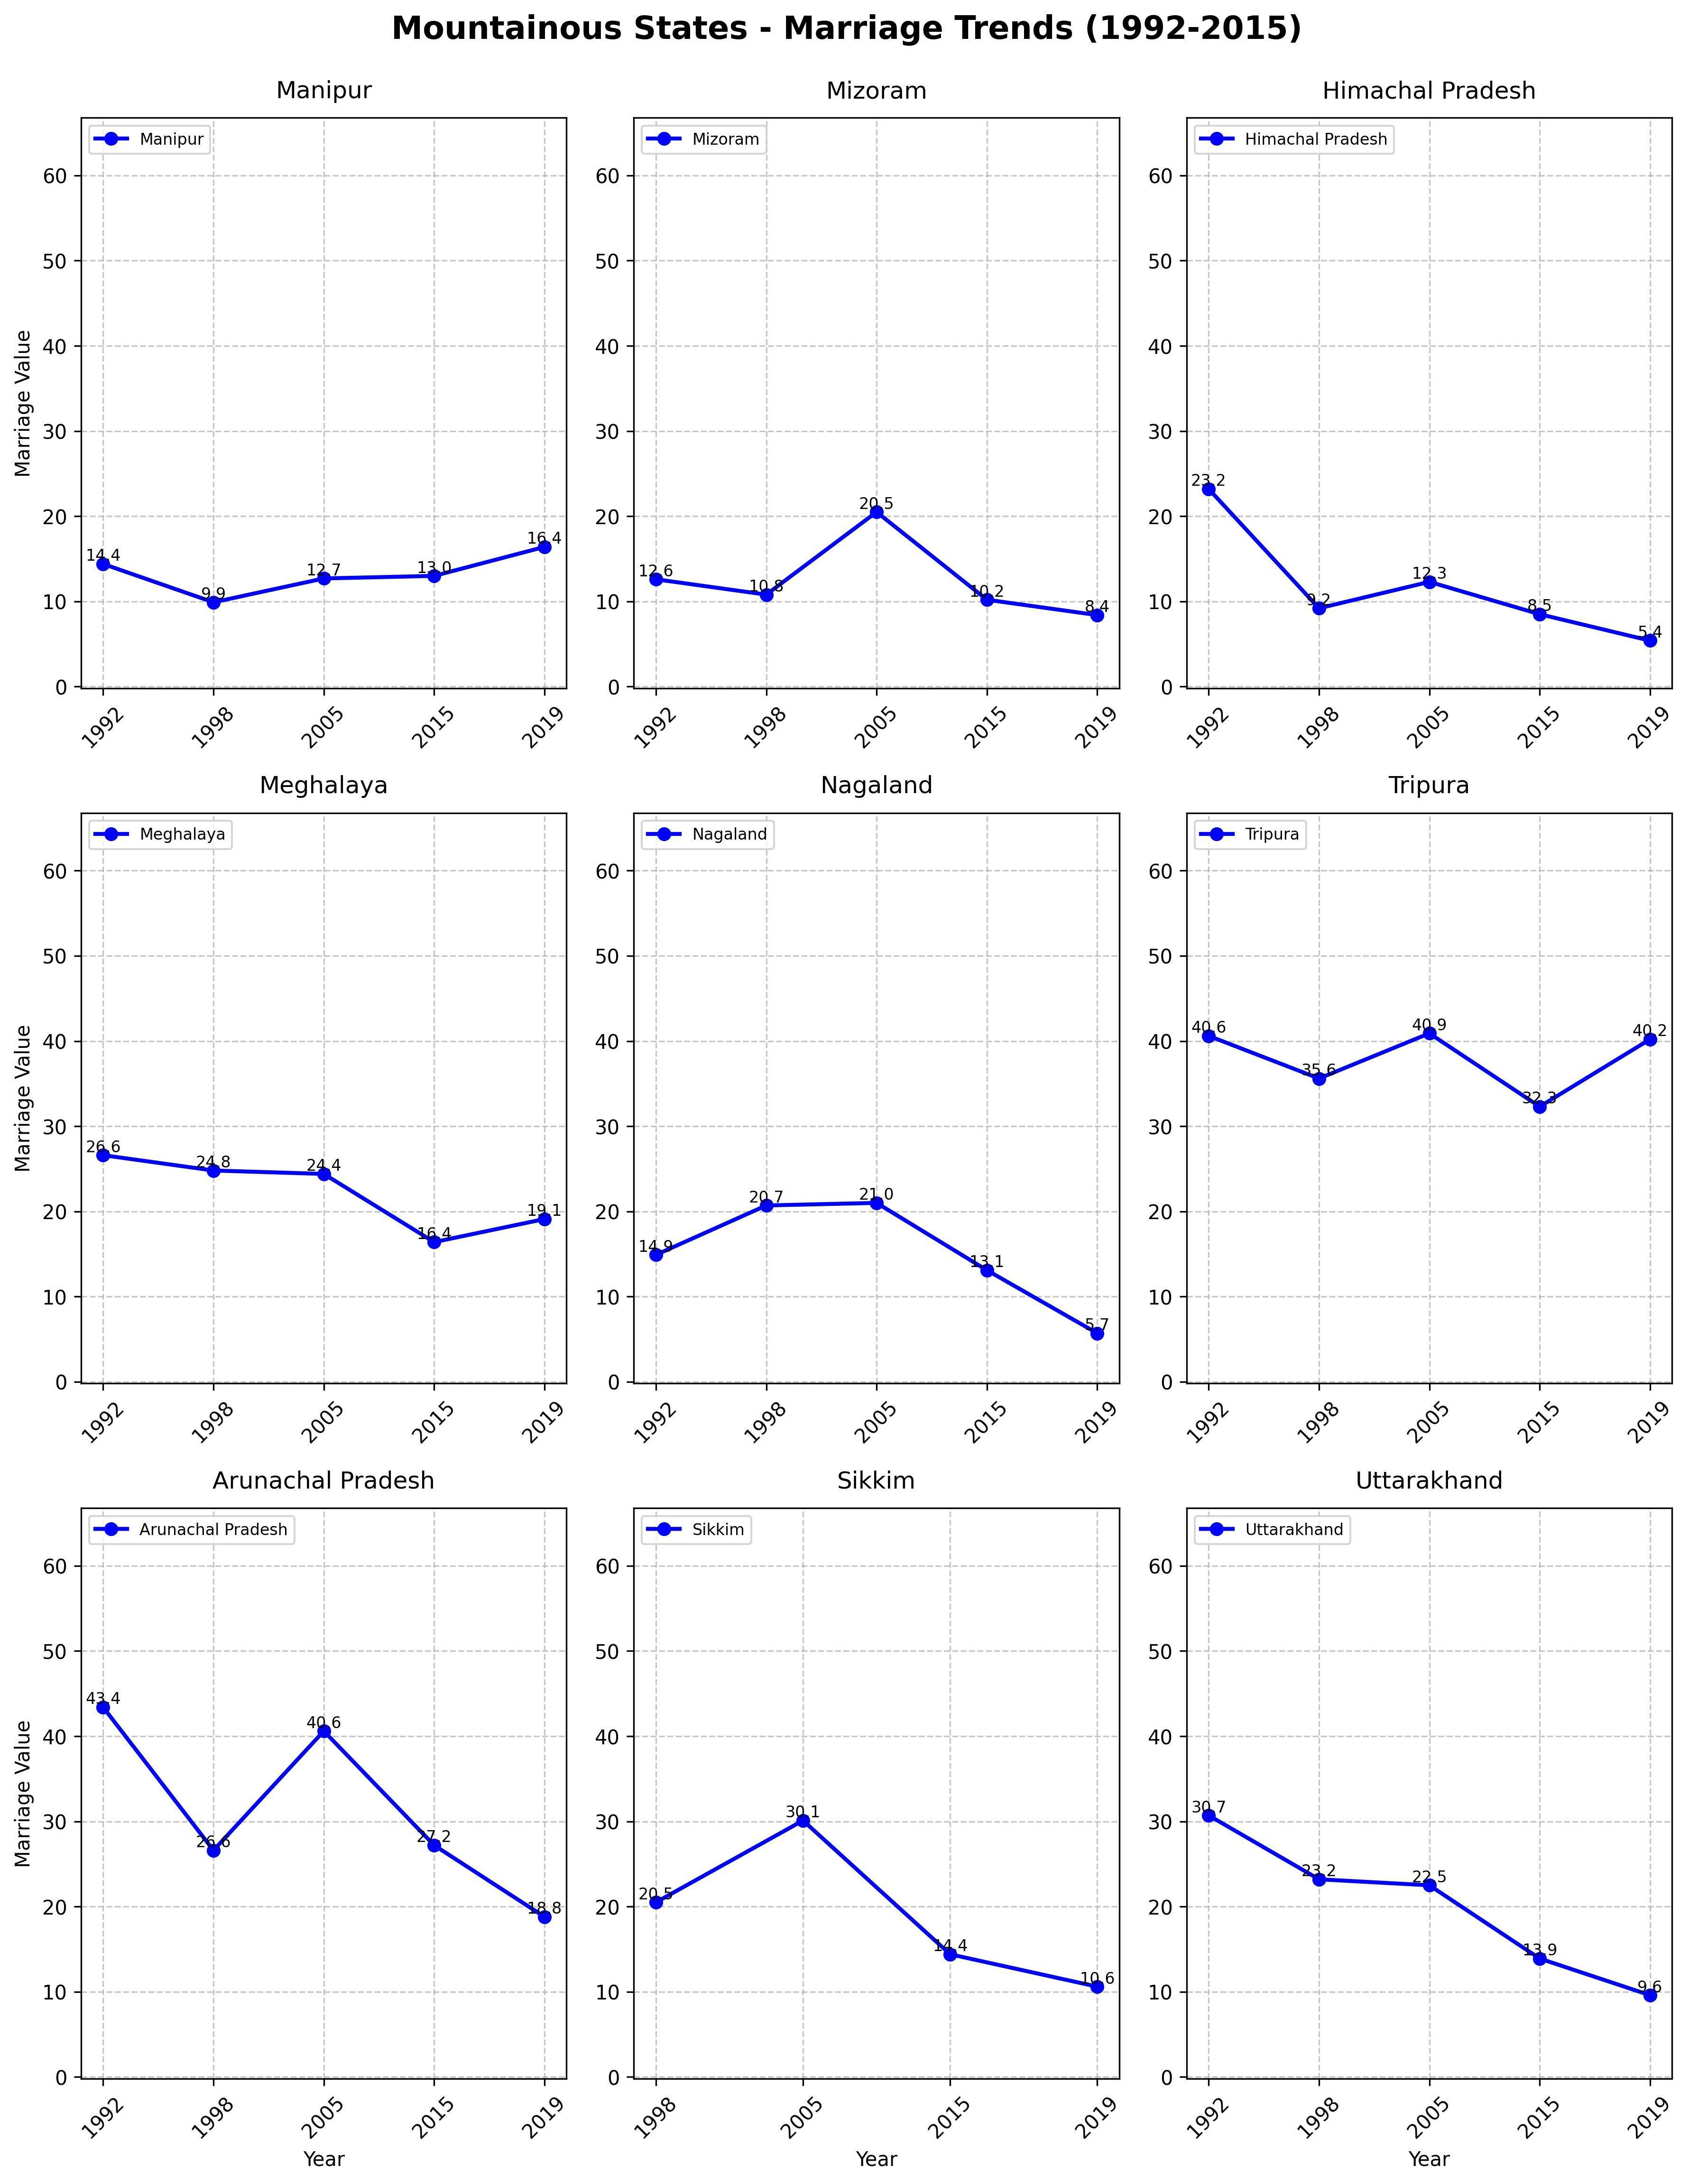
\includegraphics[width=0.9\textwidth, bb=0 0 800 800, clip]{figures/nfhs/mountainous_states_marriage_subplots.jpeg}
    \caption{Child Marriage age in Mountain States}
    \label{fig:nfhs_mountain_marriage}
\end{figure}